\section{Out of Order Execution and ILP}
We want to avoid in-order stalls so we use out of order execution to re-order instructions based on dependencies\\
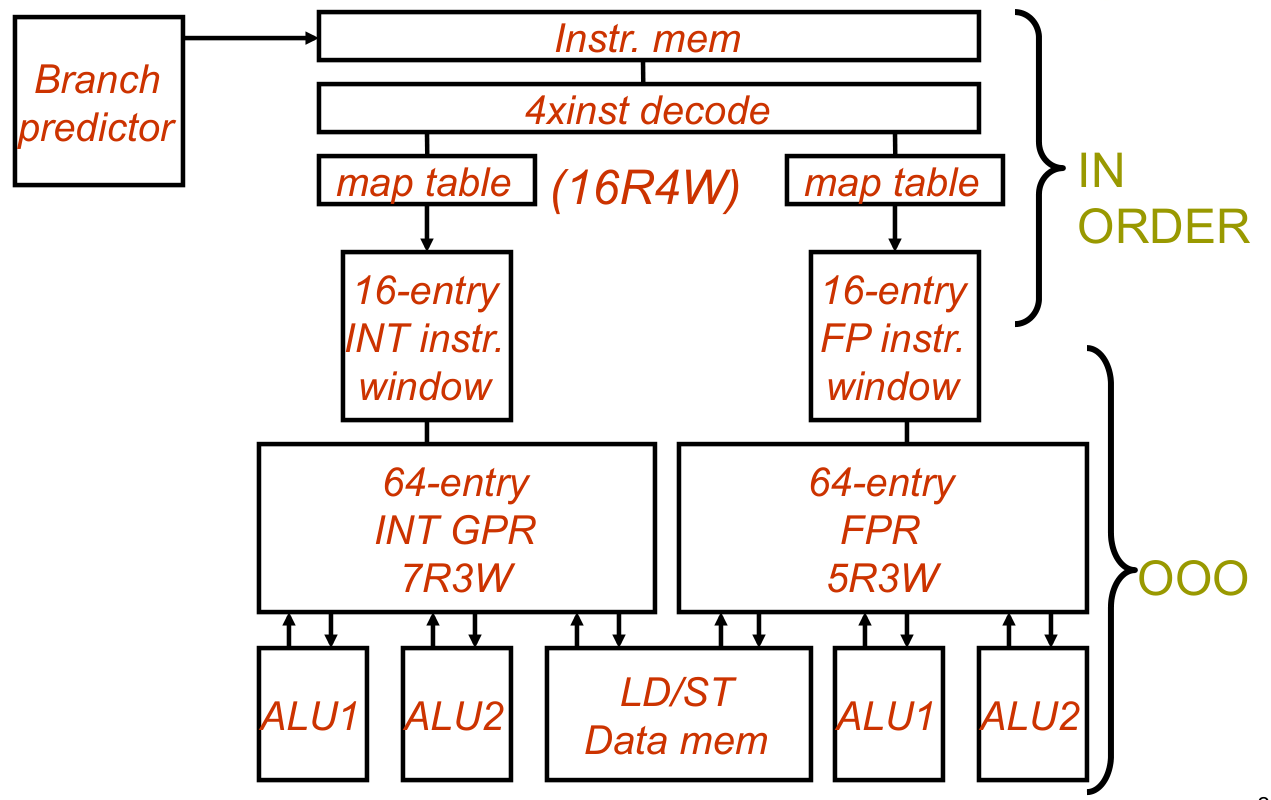
\includegraphics[width=\linewidth]{png/ooo.png}
A \textbf{superscalar processor} is a CPU that implements a form of parallelism
called instruction-level parallelism within a single processor. I.e we can launch
multiple instructions every cycle.\\

There are some issues with multiple instructions executing at onc,e we need to
double the amount of hardware, we introduce hazards, branch delay, \& load delay\\

We can rename (map) architectural registers to physical registers in decode stage
to get rid of false dependencies\\

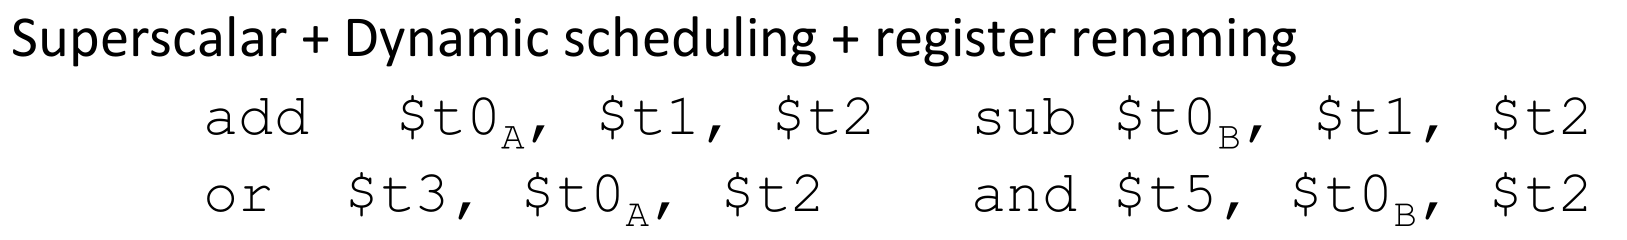
\includegraphics[width=\linewidth]{png/super.png}
There are some limits to \textbf{ILP} and pipelining:\\
Limited ILP in real programs\\
Pipeline overhead\\
Branch and load delays exacerbated\\
Clock cycle timing limits\\
Limited branch prediction accuracy (85\%-98\%)\\
Even a few percent really hurts with long/wide pipes!\\
Memory inefficiency\\
Load delays + \# of loads/cycle\\
